% draft.tex
% How Autocracy Shapes the Social Sciences: Synthetized evidence from an agent-orchestra
% Status: SKELETON — structure, tables, placeholders only. PI writes prose.

\documentclass[12pt,a4paper]{article}

% -------------------------------------------------------------------
% Packages
% -------------------------------------------------------------------
\usepackage[T1]{fontenc}
\usepackage[utf8]{inputenc}
\usepackage{lmodern}
\usepackage[margin=2.5cm]{geometry}
\usepackage{booktabs}
\usepackage{longtable}
\usepackage{array}
\usepackage{tabularx}
\usepackage{multirow}
\usepackage{hyperref}
\usepackage{setspace}
\usepackage{graphicx}
\usepackage{natbib}
\usepackage{xcolor}
\usepackage{caption}
\usepackage{subcaption}
\usepackage{amsmath}
\usepackage{amssymb}
\usepackage{pdflscape}
\usepackage{tikz}
\usetikzlibrary{arrows.meta, positioning, shapes.geometric, fit, backgrounds}

% -------------------------------------------------------------------
% Colours / notes
% -------------------------------------------------------------------
\newcommand{\todo}[1]{\textcolor{red}{[TODO: #1]}}
\newcommand{\placeholder}[1]{\textcolor{gray}{\textit{[#1]}}}
\newcommand{\kw}[1]{\textbf{#1}}

\hypersetup{
  colorlinks=true,
  linkcolor=blue!60!black,
  citecolor=blue!60!black,
  urlcolor=blue!60!black
}

% -------------------------------------------------------------------
% Title block
% -------------------------------------------------------------------
\title{\textbf{How Autocracy Shapes the Social Sciences:\\
Synthesized Evidence from an Agent Orchestra}\thanks{This research is funded by the ERC-Consolidator Project ``Authoritarian Threats to Scientific Knowledge (AUTOKNOW)'' (PI: Tore Wig), ERC-COG -- 101231399.}\\[0.5em]
\large\normalfont\textit{Preliminary draft --- please do not cite}}
\author{Tore Wig\thanks{University of Oslo. \texttt{tore.wig@stv.uio.no}}}
\date{Pre-registration date: 6 May 2026\\
\small Draft: \today}

% -------------------------------------------------------------------
\begin{document}
\maketitle
\onehalfspacing

\begin{abstract}
How does authoritarian rule shape the production of the social sciences and humanities? It is often assumed that we should observe large degrees of self-censorship and strategic content production among researchers in autocracies, in society-centered fields, yet there is little systematic evidence on this question. We look for signals of autocratic effects on social science across a wide range of different empirical implications, using an automated ``research lab"' in the form of an agent orchestra. The orchestra consists of 25 research teams (X 4 agents) that analyzes a corpus of 2.7 million SSH articles from the Web of Science, matched to data on democracy-dictatorship. Twenty-five teams of agents (designer, analyst, writer) each pre-register a distinct empirical implication of the self-censorship theory, organized into five sub-families: topic avoidance, framing neutrality, collaboration constraint, visibility suppression, and ideological alignment. In the final step we conduct a meta-analysis of the findings, discussing them in light of the overall theory. In this preliminary version we report results from 18 of the 25 teams that have completed their analyses and been reviewed. Across 18 investigations tests we find essentially no evidence of self-censorship: none of the primary coefficients on liberal democracy survives a within-family Bonferroni correction, and signs are mixed within and across sub-families.
\end{abstract}

\tableofcontents
\clearpage

% ===================================================================
\section{Introduction}
\label{sec:intro}
Autocratic regimes are increasingly making an imprint on the global production of science. China now produces more scientific articles than the United States (citation), and authoritarian countries like Saudi Arabia, Singapore and Qatar are investing heavily in academic research. How does science under autocracy differ from in a democracy? This paper considers this question in the context of the society-centered sciences, the social sciences and humanities (SSH fields). We investigate empirical implications of the assumption that we shoul dobserve significant self-censorhing behavior by SSH-researchers in autocracies, and large differences in contents across the autocracy-democracy divide.

The notion that researchers in SSH fields in autocracies should alter their behavior, regarding what they study, how they frame their findings, who they collaborate with and how visible their work becomes has a long list of different implications -- statistical signals that we should observe across a published academic work. The theory at hand thus yields a large number of different empirical implications, and it would be less informative to just focus on one. We therefore use a novel research approach that allows us to investigate several different implications under one coherent research framework: An agent-orchestra based meta-analysis. This starts from a pre-processed dataset of roughly 2,7 million SSH articles from the Web of Science (a random sample constituting around $70\%$ of the total corpus), in the period 1970-2020 for 167 countries. We then set up 25 ``research teams"', consisting of a study designer, an analyst agent, and a report writer. Each team comes up with a specific hypothesis derived from the over-arching theory that scientists react strategically to political context when doing SSH work in autocratic regimes (more so than in democracies). Each hypothesis (mechanism) is then reviewed by the PI (the lead author) and organized in theoretical sub-families, and hypotheses are pre-registered and time-stamped.\footnote{All 25 hypotheses and analysis plans were locked before any analyst session was run. Each team's pre-registration document --- including the verbal hypothesis, predicted sign, primary specification, robustness checks, and Bonferroni family --- is stored at \texttt{teams/team\_NN/preregistration.md} in the project repository at \url{https://github.com/torewig/autocracy-agent-orchestra} and is time-stamped by Git commit \texttt{960525f} (``Pre-registration: 25 teams,'' 6 May 2026). No outcome-driven changes have been made to the primary specifications since that commit.} Each team then proposes a specific design to test the respective hypotheses, and these are also reviewed and improved where needed by the PI.

The over-arching theory is driven by the core assumption that researchers will strategically alter their research behavior to minimize professional consequences relating to the regime-context they operate under. From this general assumption, we explicate five distinct families of theoretical mechanisms that can in themselves yield empirical hypotheses to be tested. These are: Topic avoidance (researchers avoid certain sensitive topics), framing neutrality (researhcers frame their work in less politically sensitive ways), collaboration constraints (researchers avoid international networks that may attract negative regime-attention), visibility suppression (that self-censored output should generate less visible work), and ideological alignment (active production of regime consonant and avoidance of regime-dissonant framings). The team then derived specific testable hypotheses for each of these families.

In the current version of this exercise, 18 teams have been reviewed, revised and completed their analysis. Across 18 tests, we find very little signals of researchers self censorship or strategic research behavior, for outcomes such as research fields, topics, abstract keywords, semantic hedging, framing neutrality, international collaboration or research visibility. The remaining tests mostly use LLMs to analyze deeper semantic dimensions of SSH contents and may yield different results, and they may use different results.  

\section{Related literature}
The impact of political regimes on academia and science more generally is a topic that has spurred much discussion across fields. In philosophy of science, it is often taken for granted that there is a link between ``open societies"' and thriving science \citep{Popper1945,kitcher2001science}. In political science, several contributions highlight how universities and academia can be in tension with autocratic regimes \citep{Dahlum19,Dahlum21,WeidmannRulis2025,Apfeld2024}, and several single-country studies focus specifically on how autocrats crack down on academia  \citep{majtenyi2025,Ertem2025,Fodor21}. A quite recent literature discusses how the new wave of authoitarian populism, signified by autocrats such as Trump, and Orban (Hungary)  antagonize and target left-leaning academic fields such as gender-studies \citep{dietze2021right}.

Political regimes (democracy-autocracy) is often studied as a determinant of scientific output, both in general \citep{Wig26} and for the social sciences and humanities more specifically \citep{Tayebi2025,Whetsell2025}. Studies indicate that the social sciences and humanities suffer pernicious effects under autocracy \citep{BerggrenBjornskov2022,Tayebi2025}. Cross-country work indicates that the democratization leads to a substantial increase in the dissemination and impact of social science research \citep{Tayebi2025}. Other studies also document positive correlations between democracy scores and greater scholarly output and citations \citet{Yang2021}.

The drop in activity and impacts in the social sciences likely reflects growing pressures on academia by autocrats. Autocrats dispose of a range of tools that can be used to crack down on and align the social sciences with their \citep{Beidollahkhani2025,Ma2023}. Autocrats can pull funding for specific fields and targeted institutional measures that ensure control. Notable examples include Russia’s 2022 announcement of the discontinuation of sociology and political science in some universities and Hungary’s expulsion of the Central European University, known for its social science focus \citep{Kosta2026,Tayebi2025}. In autocratic regime contexts, researchers must navigate blurred ``red lines’’ to avoid topics deemed politically sensitive, such as authoritarianism or public protests. Other autocratic regimes use softer tools such as state-controlled funding to incentivize research that aligns with government ideology \citep{Perry2020,Reny2016}. In China, for instance, major funding sources for the social sciences and humanities are controlled by branches of the Communist Party \citep{Holbig2014}.

In spite of this growing literature considering links between autocratic regimes and the social sciences and what and how researchers in these regimes study, the contents of social science research. If researchers actively self-censor in autocracies (compared to democracies) we should expect systematic differences in the contents and ideological lean of social science and humanities research. This is the gap we seek to fill in this study. 

By considering how autocracy affects the contents, framings and direction of the social sciences and humanities, under the driving assumption that researchers self-censor, we add to several literatures. First, we contribute to the growing political science literature on the relaitonships between autocracy-democracy and higher education and science. This is now expanding from focusing on universities as sources of dissent and liberal values \citep{Apfeld2024,Dahlum21} to how autocracy affects the intellectual products that eminate from universities. Second, we advance the ongoing discussion in the philosophy of science and science studies on how democracy matters for science \citep{Holst2026}, by showing concrete empirical results. Third, we add to the bibliometric literature that has studied the impact of regime type on scientific output volume and citations. We go beyond these measures to capture effects on deeper dimensions of scientific contents. 

% ===================================================================
\section{Theory: Self-Censorship under Autocracy}
\label{sec:theory}
% ===================================================================
We start from a set of assumptions about the motivations of researchers in the social sciences and humanities. We assume that these are driven by career incentives (to gain prominence and tenure, and get research funding) and scientific motivations (to move the literature forward and address puzzles). Furthermore, we assume that they also have to take into account the constrints placed upon them by the autocratic regime and its institutons, and act strategically within this context. While researchers want to advance their career and find things out, they also value their physical, economic and social security, and would -- ceteris paribus -- seek to avoid different types of punishment they can face from the regime. They respond rationally to both negative and positive incentive structures influenced by the regime. 

On the regime side, we assume that the ruler and his support coalition pursues political survival and want to supress threats from the opposition. To attain this, they want to minimize research dissemination and teaching that goes against official narratives and spreads potentially regime-threatening ideas relating to liberalism, democracy, human rights, minority protections and so fort, and they also want to minimize regime-criticism both direct and indirect.

The core theoretical claim is that researchers in autocracies may (relative to those in democracies) face
career costs for politically sensitive topics, methods, collaborations,
framings, and other research choices.

This broad assumption is of the kind that yields a long list of empirical implications rather than one core test. To put it in different words; researchers have an almost inumerably long list of levers to pull to subtly shape their research activity in such as way that they avoid professional consequences from the regime. Some researchers in some contexts may choose to avoid certain words, while others in other contexts refrain from engagin in international collaborations, while yet others may choose to not avoid specific topics but frame findings in a certain way. Since there allways will be some uncertainty both on the regime side and the researcher side relating to what type of content will generate a regime reaction, we expect the signals of self-censorship behavior to be wide-ranging, hard to detect, occurring in multiple different domains, and often context dependent. This particular complext of theoretical characteristic argues for testing several different implications, on many different content-outcomes rather than pursuing one unique test. 

We broadly outline five families of mechanisms that may result from the core theoretical assumption: 

\kw{Topic avoidance}: One mechanism-category has to do with researches de-prioritizing topics that (under some uncertainty) may come with regime-imposed costs. These may be topics that have to do with democratic values or democracy specifically, poor govenrance or corruption or political philosophies that engender criticism of power. The strategic behavior may occur at a very ``macro"' level, where researchers select out of entire disciplines where these topics may arise (like political science), or be more fine-grained e.g. when researchers avoid working on ``democracy"' per se. We register 7 hypotheses in this category. Examples include: That democracies  should have a higher share of political-content keywords in published articles, that democracies should produce more work in politically sensitive fields (e.g. PoliSci), that they should more often mention democracy, human rights etc., and that they should have a higher share critically examining own-country institutions. To be sure, differences across fields in different contexts may also reflect funding differences, and is therefore not solely consistent with the assumption of researcher self-censorship.  

\kw{Framing neutrality}: A second category relates to how researchers frame their findings. When there is uncertainty relating to regime-reactions, researchers may use less clear-cut language, hedge their bets, depoliticize conclusions and adopt more technocratic language in their conclusions and problem descriptions. We propose several hypotheses relating to such framing neutrality. We registered 6 hypotheses in this category, including: That autocracies should have a higher rate of ``hedging"' words in bastracts, that they should have less normative language, and a lower share ending with normative conclusions. 


\kw{Collaboration constraint}: International research networks may threaten autocratic regimes and disseminate regime-critical ideas and frameworks through research networks. If this is seen and reacted to by autocratic regimes, one would expect researchers to avoid strong international visibility, deep engagement with international networks, and particularly with partners from democratic regimes. We develop several different hypotheses that would trace this self-selection out of international networks. For example we register the hypothesis that researchers in autocracies collaborate less with researchers in democracies, have less institutional diversity in collaboration and have smaller research teams. 

\kw{Visibility suppression}: A third category relates to lowered visibility of work that is (assumed) self-censored. This arguments trades on the assumption that self-censorship acts as a perversion in the machinery of scientific output, in such a way that the work that is constrained by self-censorship is of lower quality than more uncensored work. Examples of hypotheses in this category are that autocracies should have normalized citation impact, that the citation penalty for autocracies should interact with sensitive topics, and that autocracies should have higher citation variance. 

 \kw{Ideological alignment}: In the final category of mechanisms, we present hypotheses under the assumption that researchers avoid semantic content that is dissonant with regime ideology. For example that autocracies should have a higher share of work that is higher share of work that has a neutral framing of political topics when compared to work that has a liberal political framing, that autocracies should have a higher share of work implicitly legitimating their own political system, and that they should have a higher share of work that has an anti-liberal framing.

\subsection{Pre-registered hypotheses by team}

Table~\ref{tab:hypotheses-rationale} summarises the 25 pre-registered hypotheses, organised by theory sub-family, together with a one-sentence rationale drawn from each team's pre-registration document. The full verbatim hypotheses are reproduced in Appendix~\ref{app:hypotheses-full}; the per-team design (outcome variable, controls, robustness checks) is in Appendix~\ref{app:mini-plans}.

\begin{landscape}
\small
\begin{longtable}{
  @{}
  >{\raggedright\arraybackslash}p{0.6cm}
  >{\raggedright\arraybackslash}p{3.2cm}
  >{\raggedright\arraybackslash}p{7.4cm}
  >{\raggedright\arraybackslash}p{8.4cm}
  @{}
}
\caption{Pre-registered hypotheses with theory sub-family and a one-sentence rationale (drawn from each team's \texttt{preregistration.md}).}
\label{tab:hypotheses-rationale} \\
\toprule
\textbf{T} & \textbf{Sub-family} & \textbf{Hypothesis (condensed)} &
\textbf{Rationale (one-sentence summary)} \\
\midrule
\endfirsthead
\multicolumn{4}{l}{\footnotesize\textit{(continued)}} \\
\toprule
\textbf{T} & \textbf{Sub-family} & \textbf{Hypothesis (condensed)} &
\textbf{Rationale (one-sentence summary)} \\
\midrule
\endhead
\midrule
\multicolumn{4}{r}{\footnotesize\textit{(continued on next page)}} \\
\endfoot
\bottomrule
\endlastfoot
% Auto-generated by scripts/make_hypothesis_rationale_table.R --- do not edit by hand.
% Body rows for the main-body longtable defined in draft_APSG.tex
% (label = tab:hypotheses-rationale).
01 & topic-avoidance & Countries with lower Liberal democracy levels will exhibit lower mean PCI scores in SSH abstracts. & Researchers working under autocratic rule face institutional incentives to avoid topics that may attract state scrutiny, including explicitly political subject matter. \\[3pt]
02 & topic-avoidance & Countries with lower Liberal democracy levels will exhibit lower Shannon entropy of author-supplied keyword distributions at the country-year level. & Author-supplied keywords are the researcher's own signal of what a paper is about; in autocratic settings, researchers who self-censor will gravitate toward safer, institutionally approved topics, causing keyword vocabularies to concentrate around a narrower range of terms. \\[3pt]
03 & topic-avoidance & Countries with lower Liberal democracy levels will produce a lower share of SSH output in politically sensitive disciplines. & Self-censorship does not operate only within disciplines — it also operates across them. \\[3pt]
04 & topic-avoidance & Countries with lower Liberal democracy levels will have a lower share of SSH articles containing regime-sensitive terms in titles, author keywords, and abstracts. & Self-censorship theory predicts that researchers in autocracies avoid topics that could draw state scrutiny or threaten their careers. \\[3pt]
05 & topic-avoidance & Countries with lower Liberal democracy levels will exhibit a lower share of SSH articles critically examining their own governance and institutions. & Self-censorship theories predict that researchers operating under authoritarian constraints avoid producing work that could be perceived as threatening to the regime. \\[3pt]
06 & topic-avoidance & Countries with lower Liberal democracy levels will exhibit lower mean pairwise semantic diversity of SSH abstracts within country-field-year clusters. & If researchers in autocracies self-censor by converging on politically safe topics and framings, the full semantic space of their published output — not just the presence or absence of specific keywords — should narrow. \\[3pt]
07 & topic-avoidance & Countries with lower Liberal democracy levels will have a lower share of SSH articles acknowledging international funding agencies. & Receiving funding from international agencies — such as the US National Science Foundation, the European Research Council, the World Bank, the Ford Foundation, or bilateral aid bodies — involves agreeing to donor norms, submitting to external review, and producing work that is visible to international audiences. \\[3pt]
08 & framing-neutrality & Countries with lower Liberal democracy levels will exhibit higher mean epistemic hedging rates in SSH abstracts. & Researchers working under autocratic constraints face institutional incentives not only to avoid politically sensitive topics outright, but also to hedge and soften any claims they do make, deflecting regime scrutiny by rendering findings provisional rather than declarative. \\[3pt]
09 & framing-neutrality & Countries with lower Liberal democracy levels will exhibit lower mean normative language rates in SSH abstracts. & Self-censorship theory predicts that scholars in autocracies strategically minimise language that could be read as a political or moral claim against the regime. \\[3pt]
10 & framing-neutrality & Countries with lower Liberal democracy levels will exhibit a higher share of SSH abstracts classified as purely technocratic (no political references). & Self-censorship theory predicts that researchers in autocracies will actively reframe their work to minimize the risk of regime scrutiny — not only by avoiding sensitive topics altogether, but by stripping politically referential language from work they do publish, presenting it instead in purely technical or administrative terms. \\[3pt]
11 & framing-neutrality & Countries with lower Liberal democracy levels will exhibit lower mean rates of first-person argumentative stance phrases in SSH abstracts. & Making an explicit attributed claim in academic writing ("we argue that X") exposes the author as the source of an assertion, increasing personal accountability for the content of a paper. \\[3pt]
12 & framing-neutrality & Countries with lower Liberal democracy levels will exhibit a lower share of SSH abstracts ending with an explicit normative or policy conclusion. & Self-censorship theory predicts that researchers under autocratic constraints avoid signaling political engagement. \\[3pt]
13 & framing-neutrality & Countries with lower Liberal democracy levels will publish a higher share of SSH output in domestically dominated journals. & Publishing in an international journal subjects a paper to editorial standards, reviewer networks, and professional norms anchored in liberal academic culture; publishing in a domestically dominated journal places the work in a locally controlled institutional environment where regime-aligned editorial gatekeepers have greater influence. \\[3pt]
14 & collaboration-constraint & Countries with lower Liberal democracy levels will exhibit a lower mean number of distinct co-author countries per SSH article. & International collaboration in research is not politically neutral: maintaining professional contacts abroad, exchanging manuscripts across borders, and attending international conferences all expose researchers to cross-border oversight and potential regime scrutiny. \\[3pt]
15 & collaboration-constraint & Countries with lower Liberal democracy levels will have a lower share of SSH articles co-authored with researchers from liberal democracies (v2x\_libdem > 0.5). & Collaboration with scholars in liberal democracies is not politically neutral for researchers in autocracies: democratic co-authors operate under editorial and professional norms that may encourage politically sensitive research agendas, and democratic-country affiliations may trigger regime suspicion toward the collaboration and its outputs. \\[3pt]
16 & collaboration-constraint & Countries with lower Liberal democracy levels will exhibit a higher share of SSH articles with exclusively domestic authorship. & Self-censorship theory predicts that researchers in autocracies constrain their collaboration choices to minimize exposure to foreign oversight, documentation of foreign contacts, and the transmission of liberal academic norms. \\[3pt]
17 & collaboration-constraint & Countries with lower Liberal democracy levels will exhibit a lower mean number of authors per SSH article. & Collaborative research requires multiple people to share ideas, access data, and jointly produce work that may attract political scrutiny. \\[3pt]
18 & collaboration-constraint & Countries with lower Liberal democracy levels will exhibit a lower mean number of distinct author institutions per SSH article. & Inter-institutional collaboration requires spreading a research project across organizational boundaries — across universities, research centers, government agencies, and other bodies. \\[3pt]
19 & visibility-suppression & Countries with lower Liberal democracy levels will exhibit a lower mean normalized citation ratio for SSH articles. & Self-censorship produces work that is rhetorically cautious, topically narrow, and unlikely to engage the politically salient debates that drive citation traffic in SSH; hedged claims and depoliticized framings give other scholars little to build on, criticize, or extend, so on average autocracy-produced SSH work should attract fewer citations than comparable work from democratic contexts. \\[3pt]
20 & visibility-suppression & The citation penalty associated with lower Liberal democracy levels will be larger for politically sensitive articles than for non-sensitive articles, as indicated by a positive coefficient on the v2x\_libdem × sensitive\_flag interaction term. & If self-censorship operates through cautious framing and weakened claims, the citation penalty should not apply uniformly: politically non-sensitive SSH topics impose few framing constraints in either regime context, so citations should be comparable, while sensitive topics force autocratic authors to hedge, depoliticize, or narrow their contributions in ways their democratic counterparts are not constrained to do --- producing a citation gap that concentrates precisely where the theory predicts self-censorship bites hardest. \\[3pt]
21 & visibility-suppression & Countries with lower Liberal democracy levels will exhibit a lower share of SSH articles that receive at least one citation within a country-year. & Articles that fail to advance any distinctive claim are the ones most likely to attract zero citations; if self-censorship pushes researchers toward incremental, low-stakes contributions on safe topics, autocratic SSH output should exhibit a larger share of articles that never enter scholarly conversation at all. This is the extensive-margin counterpart to the average-impact test in Team 19. \\[3pt]
22 & visibility-suppression & Countries with lower Liberal democracy levels will exhibit a higher Gini coefficient of citations across SSH articles. & Self-censorship may bifurcate autocratic SSH output: a small set of articles --- those touching on regime-endorsed priorities, applied development topics, or internationally co-funded projects --- escape the constraints and accumulate citations normally, while the conformist majority is undifferentiated and rarely cited. Citation distribution within autocratic country-years should therefore be more skewed than in democratic ones, captured by a higher within-cell citation Gini. \\[3pt]
23 & ideological-alignment & Countries with lower Liberal democracy levels will exhibit a lower share of SSH abstracts with liberal/neutral political-economy framing (NEUTRAL + NONE) and a higher share with ideologically aligned framing (LEFT or RIGHT-CONSERVATIVE). & Self-censorship under autocracy is not ideologically neutral: researchers in communist regimes face pressure to produce scholarship consonant with statist, collectivist, and anti-market frames, while researchers in nationalist or right-authoritarian regimes face complementary pressures toward market-nationalist or traditionalist frames. \\[3pt]
24 & ideological-alignment & Countries with lower Liberal democracy levels will exhibit a higher share of SSH abstracts that actively legitimize or endorse the current political system, state authority, or leadership. & Self-censorship theories have largely focused on what researchers avoid; yet autocratic regimes do not merely suppress dissent — they actively incentivize, fund, and reward scholarship that validates state power and ideology. \\[3pt]
25 & ideological-alignment & Countries with lower Liberal democracy levels will exhibit a higher share of SSH abstracts that actively frame liberal democracy, Western political institutions, or international human rights norms as fundamentally flawed or illegitimate. & Self-censorship theory predicts that researchers in autocracies avoid politically sensitive topics to minimize career risk, but the same logic of regime alignment generates an additional prediction: where states actively promote counter-liberal ideologies, researchers face positive incentives to produce scholarship consonant with those ideologies. \\[3pt]

\end{longtable}
\end{landscape}

\subsection{Hypotheses and significance thresholds}
Table~\ref{tab:families} lists the five theory sub-families, the teams
assigned to each, and the Bonferroni-corrected significance threshold for each family.

\begin{table}[ht]
\centering
\caption{Theory families, team assignments, and Bonferroni thresholds}
\label{tab:families}
\begin{tabular}{llcc}
\toprule
Sub-family & Teams & $k$ & Adjusted $\alpha$ ($0.05/k$) \\
\midrule
topic-avoidance          & 01--07 & 7 & $p < 0.0071$ \\
framing-neutrality       & 08--13 & 6 & $p < 0.0083$ \\
collaboration-constraint & 14--18 & 5 & $p < 0.0100$ \\
visibility-suppression   & 19--22 & 4 & $p < 0.0125$ \\
ideological-alignment    & 23--25 & 3 & $p < 0.0167$ \\
\midrule
\textbf{Total}           & 01--25 & \textbf{25} & \\
\bottomrule
\end{tabular}
\end{table}

The condensed hypotheses + rationale summary above are in Table~\ref{tab:hypotheses-rationale}; verbatim hypotheses are in Appendix~\ref{app:hypotheses-full}.

\section{Methodological approach: Synthetized evidence from an AI-agent orchestra}
The approach taken in this paper is unconventional. Rather than proposing and elobaring on a detailed research design testing one specific implication of the theory, and working as hard as possible to shore up the causal assumptions of that specific design, we take an approach that is more capable of accomodating information from several different tests across a wide range of outcome variables; the classic domain of meta-analysis. More specifically, we set up an AI agent orhcestra (using ClaudeCode, and Anthropic's Opus and Sonnet models) that collaborates with and is overseen by the Principal Investigator (lead author) in several steps. The orchestra consists of 25 ``research teams"' consisting of i) a study designer that develops a clear hypothesis, and proposes an analysis plan, ii) an data analyst that executes the pre-registered analysis in R, a iv) Writer that drafts up a short research report of the findings, a iii) reviewer that provides feedback on the report, and a synthesizer that models cross-team theory agreement using Bayesian synthesis. In each step, the PI is providing feedback, redirecting the team, reviewing code and results, and proposes new directions. This is a classic case of ``agent-orchestration"' which is developing as a new methodology in social science data analysis \citep{zhu2026hler,gupta2026accelerating}. 

The approach is described in greater detail below. But it requires a more in-depth justification here. Why use this approach when more standard approaches are available? First, this is a highly useful method for the specific purpose at hand, which is to test a theory that has an almost inumerable number of concrete empirical implications, none of which sit directly at the core of the theoretical logic of self-censorship (this is consistent with several different and substitutable behaviors). The core theoretical mechanism (researcher self-censorship and strategic behavior) is unobservable, and the many behaviors that are consistent with it and thus the potential universe of statistically observable signals in published work, almost infinite. Second, it is a low-cost way to push the research frontier on a ``research project"' scale with relatively low investment. Investigating a large number of hypotheses with heavy-duty data analysis would require a medium-sized research team of several postdocs and PhDs working over a long period. Using an agent-orchestra speeds and scales up this process, providing plausibly similar results. Third, the chosen approach here includes a heavy emphasis on ``human in the loop"' elements, where the lead author (as PI) reviews all the code, provides feedback on all analysis plans and quality checks all output, in the same way as a lead researcher would do on a research project leading a team of junior scholars. 

The approach undoubtedly comes with downsides. First, it means that some of the input to the project (e.g. design proposals, coding decisions, operationalizations, etc. comes from AI), which can hallucinate and make unsupervised mistakes. To ameliorate these issues, the PI has read and tested the code, and supervised all stages of the process. All elements of the analysis is verified by the PI and can be replicated from the raw data. To ensure full transparency, all code, all prompts and agent-steering documents, and all analysis logs and pre-analysis plans are available on github. 


% ===================================================================
\section{Data and Corpus}
\label{sec:data}
% ===================================================================
All teams work from the same data source, which is a bibliometric corpus of articles registered in the Web of Science (downloaded from Web of Science through their API in 2021, by the PI and co-authors). This corpus is then filtered on social science and humanities articles (by the field-categories listed in the web of science and noted on each article). The final corpus includes 2,709,224 SSH articles, in the years 1970-2023. Each article is then broken down into article-rows that can be assigned to countries. When articles are co-authored, we count each co-authoring country as 1 article for that country. All articles contain information on title, publication time, abstract, journal, subject keywords, field classification, institutions of the authors and addresses. These addresses are matched to countries with a very high success rate. 

These article-data are then matched to information on political regimes, using the Varieties of Democracy dataset \citep{Coppedge2024}. As the main predictor variable we use the Liberal Democracy index, which should most closely line up with the theory that relates to academic self-censorship based on threats to free speech and professional sanctions. The liberal democracy index emphasizes civil rights and free speec (and academic freedom) in addition to the core electoral components of democracy and is thus well suited as our main independent vairable. It ranges between 0 and 1. As an alternative regime indicator we use the Lexical Index of Democray \citep{skaaning2015lexical} in robustness tests. We also provide a set of standard controls, that each team will use, log(Gdp per capita) and log(population)

To make sure that we are not just capturing differences between those countries that publish nothing in a given field and those that publish more than 0, we preprocess the data to only include countries that publish at least 10 articles in the SSH corpus in a given year. The article corpus data, with the above listed variables, is fully locked prior to any analysis and can not be manipulated by the agents.
 
% ===================================================================
\section{Agent-Orchestra Methodology}
\label{sec:method}
% ===================================================================

\subsection{Pipeline overview}
The multi-agent pipeline consists of five sequential agent
types. Each team is assigned one instance of each agent. All designs
are pre-registered before any analysis is run.

Figure~\ref{fig:pipeline} illustrates the full pipeline.

% Colour palette for the pipeline figure (declared at document scope so
% \resizebox doesn't treat them as content).
\definecolor{agentblue}{RGB}{31,97,163}
\definecolor{gateamber}{RGB}{200,120,20}
\definecolor{milestoneteal}{RGB}{20,140,110}
\definecolor{synthviolet}{RGB}{110,50,160}
\definecolor{lightgray}{RGB}{240,240,240}

% The full pipeline (9 nodes plus phase brackets and legend) is ~27cm
% wide at its designed sizes; that overflows a portrait page by ~14cm.
% Rotating to landscape via pdflscape + scaling the tikz uniformly to
% fit \linewidth keeps the diagram readable.  We avoid the figure float
% (which would escape \begin{landscape}) and use \captionof{figure}
% from the caption package for numbering instead.
\begin{landscape}
\begin{center}
\resizebox{\linewidth}{!}{%
\begin{tikzpicture}[
  %--- node styles ---
  agent/.style  = {rectangle, rounded corners=4pt,
                   draw=agentblue, fill=agentblue!12, thick,
                   text=agentblue!80!black, font=\small\bfseries,
                   minimum width=2.3cm, minimum height=0.85cm,
                   align=center},
  gate/.style   = {diamond, aspect=2.2,
                   draw=gateamber, fill=gateamber!15, thick,
                   text=gateamber!80!black, font=\small\bfseries,
                   inner sep=1pt, align=center},
  mile/.style   = {rectangle, rounded corners=3pt,
                   draw=milestoneteal, fill=milestoneteal!12, thick,
                   text=milestoneteal!80!black, font=\small\bfseries,
                   minimum width=2.5cm, minimum height=0.85cm,
                   align=center},
  synth/.style  = {rectangle, rounded corners=4pt,
                   draw=synthviolet, fill=synthviolet!12, thick,
                   text=synthviolet!80!black, font=\small\bfseries,
                   minimum width=2.3cm, minimum height=0.85cm,
                   align=center},
  sub/.style    = {font=\scriptsize, text=black!60, align=center},
  arr/.style    = {-{Stealth[length=6pt]}, thick, black!50},
  %--- positioning ---
  node distance = 0.55cm and 0.65cm,
]

% === Row 1: main pipeline (left to right) ===
\node[agent]   (des)  {Designer};
\node[gate,    right=of des]   (gB)   {Gate B\\(PI)};
\node[mile,    right=of gB]    (prereg) {Pre-\\registration};
\node[agent,   right=of prereg](ana)  {Analyst};
\node[gate,    right=of ana]   (gD)   {Gate D\\(PI)};
\node[agent,   right=of gD]    (wri)  {Writer};
\node[gate,    right=of wri]   (gG)   {Gate G\\(PI)};
\node[agent,   right=of gG]    (rev)  {Reviewer};
\node[synth,   right=of rev]   (syn)  {Synthesizer};

% === Sub-labels (session counts / notes) ===
\node[sub, below=0.18cm of des]    {25 sessions};
\node[sub, below=0.35cm of gB]     {approve /\\redirect};
\node[sub, below=0.18cm of prereg] {GitHub commit\\(locked)};
\node[sub, below=0.18cm of ana]    {25 sessions\\(R analysis)};
\node[sub, below=0.35cm of gD]     {approve /\\redirect};
\node[sub, below=0.18cm of wri]    {25 sessions\\(8-sec report)};
\node[sub, below=0.35cm of gG]     {approve /\\revise};
\node[sub, below=0.18cm of rev]    {25 sessions\\(peer review)};
\node[sub, below=0.18cm of syn]    {1 session\\(theory eval.)};

% === Arrows ===
\draw[arr] (des)    -- (gB);
\draw[arr] (gB)     -- (prereg);
\draw[arr] (prereg) -- (ana);
\draw[arr] (ana)    -- (gD);
\draw[arr] (gD)     -- (wri);
\draw[arr] (wri)    -- (gG);
\draw[arr] (gG)     -- (rev);
\draw[arr] (rev)    -- (syn);

% === Dashed feedback loops from gates ===
% Tight horizontal gap (~0.65 cm) between each Agent and Gate, so a flat
% `bend left' arc is invisible.  Force a tall U-shaped arc above the
% nodes via explicit out/in angles plus high looseness, and put a
% white-filled label on top of the arc so it does not collide with the
% solid forward arrow below.
\tikzset{
  fbarr/.style = {-{Stealth[length=5pt]}, dashed, gateamber!85, thick},
  fblabel/.style = {midway, above, font=\scriptsize,
                    text=gateamber!80!black,
                    fill=white, inner sep=1pt, inner ysep=0pt}
}
\draw[fbarr] (gB.north) to[out=110, in=70, looseness=2.6]
      node[fblabel] {redesign} (des.north);
\draw[fbarr] (gD.north) to[out=110, in=70, looseness=2.6]
      node[fblabel] {revise} (ana.north);
\draw[fbarr] (gG.north) to[out=110, in=70, looseness=2.6]
      node[fblabel] {revise} (wri.north);

% === Phase bracket labels ===
% Phases 1A, 1B and 2 each contain a dashed feedback arc above the nodes,
% so they get a taller `inner ysep' to keep the arc inside the bracket.
% Pre-reg, Phase 3 and Phase 4 have no feedback arc and keep the tight default.
\begin{scope}[on background layer]
  % Phase 1A
  \node[draw=agentblue!30, fill=agentblue!4, rounded corners=3pt,
        fit=(des)(gB), inner xsep=6pt, inner ysep=14pt,
        label={[font=\tiny\color{agentblue},
        anchor=south]above:Phase 1A}] {};
  % Phase 1B
  \node[draw=milestoneteal!30, fill=milestoneteal!4, rounded corners=3pt,
        fit=(prereg), inner sep=6pt, label={[font=\tiny\color{milestoneteal},
        anchor=south]above:Pre-reg}] {};
  % Phase 1C
  \node[draw=agentblue!30, fill=agentblue!4, rounded corners=3pt,
        fit=(ana)(gD), inner xsep=6pt, inner ysep=14pt,
        label={[font=\tiny\color{agentblue},
        anchor=south]above:Phase 1B}] {};
  % Phase 2
  \node[draw=agentblue!30, fill=agentblue!4, rounded corners=3pt,
        fit=(wri)(gG), inner xsep=6pt, inner ysep=14pt,
        label={[font=\tiny\color{agentblue},
        anchor=south]above:Phase 2}] {};
  % Phase 3
  \node[draw=agentblue!30, fill=agentblue!4, rounded corners=3pt,
        fit=(rev), inner sep=6pt, label={[font=\tiny\color{agentblue},
        anchor=south]above:Phase 3}] {};
  % Phase 4
  \node[draw=synthviolet!30, fill=synthviolet!4, rounded corners=3pt,
        fit=(syn), inner sep=6pt, label={[font=\tiny\color{synthviolet},
        anchor=south]above:Phase 4}] {};
\end{scope}

% Legend removed (was a TikZ matrix that interacted badly with \resizebox
% and the colour key is already in the caption below).

\end{tikzpicture}%
}% end \resizebox
\captionof{figure}{Agent-orchestra pipeline. \textbf{Blue}: agent sessions (Claude Sonnet/Haiku);
\textbf{amber}: PI gate reviews; \textbf{teal}: pre-registration milestone;
\textbf{violet}: synthesis. Dashed arrows indicate redesign/revision loops possible at each gate.
Current status: pre-registration complete (gate B passed); analyst sessions pending.}
\label{fig:pipeline}
\end{center}
\end{landscape}

\subsection{Agent roles}

Each team runs four agents in sequence. The \textbf{Designer} develops the
research question, operationalization, and analysis plan within a
pre-assigned theoretical domain, producing \texttt{rq.md} and
\texttt{analysis\_plan.md}. The \textbf{Analyst} executes the
pre-registered analysis in R against the locked corpus and writes
\texttt{analysis.R}, the figures, and a machine-readable
\texttt{primary\_results.json}. The \textbf{Writer} drafts the team report
following a standardized 8-section template
(\texttt{report.md}), and the \textbf{Reviewer} --- a separate agent
instance --- peer-reviews that report against rubric criteria
(\texttt{peer\_review.md}).

Once all 25 teams have completed this pipeline, the PI reads all reports, then aggregates the sub-family verdicts, then discusses these in light of the theory.

\subsection{Pre-registration}

All 25 teams' hypotheses and analysis plans were committed to GitHub
(commit \texttt{960525f}) on 6 May 2026, before any analyst session was run.
The timestamp and Git commit hash constitute the pre-registration record.
Bonferroni adjustment is computed programmatically post-analysis using
\texttt{scripts/bonferroni\_adjust.R}.

\subsection{Estimation strategy}
Each team is instructed to follow a set estimation strategy for their primary specification, since all teams analyze the data (the treatment) at the country-level. Crucially we instruct them to estimate Two-way fixed effects (TWFE):
\begin{equation}
  Y_{it} = \beta \cdot \texttt{Liberal democracy}_{it}
           + \gamma_1 \log(\texttt{gdppc}_{it})
           + \gamma_2 \log(\texttt{pop}_{it})
           + \alpha_i + \delta_t + \varepsilon_{it}
\end{equation}
where $\alpha_i$ = country FE, $\delta_t$ = year FE, SE clustered by \texttt{iso3}.

They can also supplement this analysis with a less strict specification, which is a ``pooled"' model with 
Year FE only (no country FE), SE clustered by \texttt{iso3}. This checks whether
the within-country estimate is consistent with the cross-sectional pattern and tells us about average differences between democracies and dictatorships, rather than how SSH publications change their content as a function of variation in democracy-autocracy over time. 

\paragraph{Robustness checks.} All teams are instructed to specify two core robustness tests, that are proposed to the PI and revised on demand. 

% ===================================================================
% ===================================================================
\section{Current stage}
\label{sec:current-stage}
% ===================================================================

The project follows the agent-orchestra pipeline of
Figure~\ref{fig:pipeline}: per team, a deterministic Designer ---
Analyst --- Writer --- Reviewer sequence punctuated by PI review gates
(B, D, G), with a single Synthesizer pass at the end that aggregates
across all 25 teams. As of this draft, Phase~0 (data preparation) and
Phase~1A (the 25 Designer sessions) are complete, Gate~B was passed on
6~May 2026, and all 25 hypotheses and analysis plans have been
pre-registered on GitHub at commit \texttt{960525f}. The corpus
(\texttt{data/agent\_corpus.rds}, 2{,}709{,}224 articles) has been
locked since before any analyst session and is not modified downstream.

Phase~1B (Analyst sessions) is partially complete: 18 of the 25 teams
that rely only on the bibliometric corpus and V-Dem have finished their
pre-registered analyses, with results reported in
Section~\ref{sec:results}. The remaining seven teams --- 05, 06, 10,
12 (LLM and embedding teams in the topic-avoidance and
framing-neutrality families) and 23--25 (the entire
ideological-alignment family) --- depend on external classifier or
embedding API calls and are queued pending budget sign-off. Gate~D
(PI review of all 25 result sets), Phase~2 (Writer sessions), Gate~G,
Phase~3 (Reviewer sessions), and Phase~4 (Synthesis) are all blocked
downstream of the remaining seven analyses. A full disposition with
per-phase outputs, gate criteria, and the agent sessions still to run
is given in Appendix~\ref{app:disposition}.

% ===================================================================
\section{Results}
\label{sec:results}
% ===================================================================

\subsection{Coverage so far}

Of the 25 pre-registered teams, \textbf{18 have completed analyst
sessions} at the time of writing: all teams in the topic-avoidance,
framing-neutrality, collaboration-constraint, and visibility-suppression
sub-families that rely only on the bibliometric corpus and V-Dem.
The remaining \textbf{seven teams} --- 05, 10, 12 (LLM classifiers of
framing), 06 (text embeddings), and 23--25 (the entire
ideological-alignment sub-family, LLM classifiers of regime-consonant
content) --- require external API calls and are queued pending budget
sign-off. Section~\ref{sec:results} therefore reports a preliminary
snapshot covering 18 of 25 pre-registered implications, organized by
the four sub-families for which results are currently in.

\subsection{Main coefficients by sub-family}

Figure~\ref{fig:main-coef} summarizes the primary estimate from each of
the 18 completed teams. Each row is one team's pre-registered test:
the point is the standardized estimate $\hat{\beta}/\widehat{\mathrm{SE}}$
of the coefficient on \texttt{v2x\_libdem} from the TWFE specification
(country and year fixed effects, log GDP per capita and log population
as controls, standard errors clustered by country), and the horizontal
bar is the 95\% confidence interval in the same standardized scale.
The dashed vertical lines mark the nominal $\pm 1.96$ threshold; the
dotted lines mark the family-specific Bonferroni-corrected 5\%
threshold ($\alpha = 0.05/k$ within each sub-family).

\begin{figure}[ht]
\centering
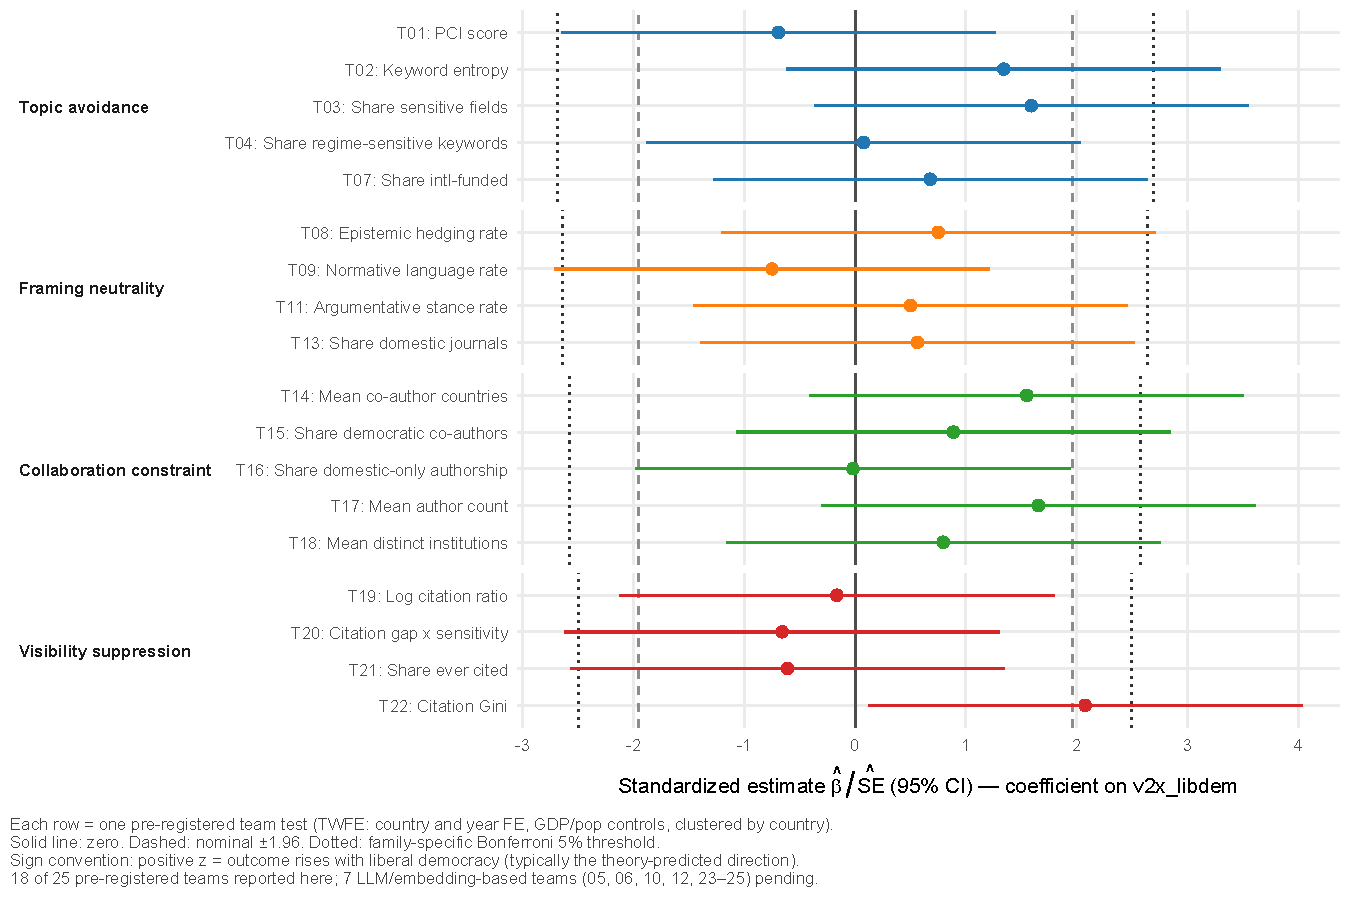
\includegraphics[width=\textwidth]{figures/fig_main_coefficients.pdf}
\caption{Main coefficients on \texttt{v2x\_libdem} for the 18 completed
teams, organized by theory sub-family. Standardized as
$\hat{\beta}/\widehat{\mathrm{SE}}$ with 95\% confidence intervals.
Solid line: zero. Dashed: nominal $\pm 1.96$. Dotted: family-specific
Bonferroni 5\% threshold. Positive values indicate that the outcome
rises with liberal democracy, which corresponds to the
theory-predicted direction for most --- but not all --- teams (see
each team's \texttt{preregistration.md} for the expected sign).}
\label{fig:main-coef}
\end{figure}

The pattern across the 18 tests is clear: \textbf{no team's primary
coefficient survives its family-specific Bonferroni threshold}, and only
one team (Team 22, citation Gini) clears the nominal $p<0.05$ line. Even
that single nominal exception goes in the \emph{opposite} direction to
its hypothesis. Within sub-families, signs are mixed for topic avoidance
and framing neutrality; the four collaboration-constraint estimates
(Teams 14, 15, 17, 18) all point in the theory-predicted direction but
none of them reaches significance; the visibility-suppression estimates
match the predicted sign but cluster tightly around zero.

\subsection{Synthesis across sub-families}

Table~\ref{tab:meta-summary} aggregates the 18 completed tests by theory
sub-family. Across all four families, no primary coefficient survives its
family-specific Bonferroni threshold, and only one of the 18 tests reaches
nominal significance; coefficient signs are split 12 to 6 across the completed
teams.

\begin{table}[ht]
\centering
\caption{Synthesis of the 18 completed team tests, by theory sub-family.}
\label{tab:meta-summary}
% Auto-generated by scripts/make_meta_summary_table.R - do not edit by hand.
\begin{tabular}{@{}l c c c c c c@{}}
\toprule
 & Registered & Completed & \multicolumn{2}{c}{Sign of $\hat{\beta}$} & Nominal & Bonferroni \\
\cmidrule(lr){4-5}
Sub-family & ($k$) & tests & $>0$ & $<0$ & $p<.05$ & $p<.05$ \\
\midrule
Topic avoidance & 7 & 5 & 4 & 1 & 0 & 0 \\
Framing neutrality & 6 & 4 & 3 & 1 & 0 & 0 \\
Collaboration constraint & 5 & 5 & 4 & 1 & 0 & 0 \\
Visibility suppression & 4 & 4 & 1 & 3 & 1 & 0 \\
\midrule
\textbf{Total} & \textbf{22} & \textbf{18} & \textbf{12} & \textbf{6} & \textbf{1} & \textbf{0} \\
\bottomrule
\end{tabular}


\vspace{0.4em}
{\footnotesize\begin{minipage}{0.92\textwidth}
\emph{Notes:} One row per sub-family. ``Registered ($k$)'' is the
pre-registered number of tests in the family, which serves as the fixed
Bonferroni denominator; ``Completed'' is the number of those tests reporting at
the time of writing. ``Sign of $\hat{\beta}$'' counts the direction of each
team's primary coefficient on \texttt{v2x\_libdem}. ``Nominal $p<.05$'' counts
tests with raw $p<0.05$; ``Bonferroni $p<.05$'' counts tests whose adjusted
$p$-value ($p_{\text{adj}} = \min(p \times k,\,1)$) falls below $0.05$. The
three pre-registered ideological-alignment teams (23--25) are still queued and
are omitted here.
\end{minipage}}
\end{table}


% ===================================================================
\section{Discussion}
\label{sec:discussion}
This paper presents a synthesized meta-analysis of the question of whether autocracies lead researchers to change their publication behavior. Using an AI-agent orchestra we look for statistical traces of researchers strategic behavior under autocracy in a corpus of over 2,7 million published social sciences and humanities articles. The orchestra tests 25 pre-registered hypotheses relating to topic choice, framing neutrality, international research collaboration, scientific visibility, and ideological alignment. The current status of the project has finalized 18 team reports, documenting no evidence of researcher's strategic behavior under autocracy. The next stage of the project will complete the more LLM-heavy semantic analyses of ideological alignments etc. and then evaluate the overall synthesis. 
% References
% ===================================================================
\clearpage
\bibliographystyle{apsr}
\bibliography{autocrat}
% \todo{Build references.bib}

% ===================================================================
% Appendix
% ===================================================================
\appendix

\section{Team roster and file map}
\label{app:teams}

\begin{table}[ht]
\centering
\caption{Team file structure (one row per team)}
\label{tab:filemap}
\small
\begin{tabular}{@{}lllll@{}}
\toprule
Team & Sub-family & \texttt{rq.md} & \texttt{analysis\_plan.md} & \texttt{preregistration.md} \\
\midrule
01--07  & topic-avoidance          & \checkmark & \checkmark & \checkmark \\
08--13  & framing-neutrality       & \checkmark & \checkmark & \checkmark \\
14--18  & collaboration-constraint & \checkmark & \checkmark & \checkmark \\
19--22  & visibility-suppression   & \checkmark & \checkmark & \checkmark \\
23--25  & ideological-alignment    & \checkmark & \checkmark & \checkmark \\
\bottomrule
\end{tabular}
\end{table}

\section{Project disposition (full)}
\label{app:disposition}

This appendix gives the full per-phase project disposition. Section~\ref{sec:current-stage} summarises the headline status; the inputs, outputs, gate criteria and pending sessions for each phase appear here.

\subsection*{Phase 0 --- Data preparation (Complete)}

\begin{itemize}
  \item Raw WOS SSH records downloaded and parsed: 3,189,557 rows
  \item De-duplicated to 2,709,224 unique articles (\texttt{wos\_id})
  \item V-DEM political data merged at \texttt{iso3} $\times$ \texttt{year} level
  \item Country coverage: 99.98\% match rate
  \item Controls added: log GDP per capita, log population
  \item Output: \texttt{data/agent\_corpus.rds} (locked; not tracked in Git)
\end{itemize}

\subsection*{Phase 1A --- Designer sessions (Complete)}

\begin{itemize}
  \item 25 Designer agent sessions run (Claude Sonnet)
  \item Each session: read brief + data description, develop RQ within domain
  \item Output: \texttt{rq.md} + \texttt{analysis\_plan.md} per team
  \item Uniqueness check enforced: no two teams share outcome + unit + strategy
\end{itemize}

\subsection*{Gate B --- PI review (Complete, 6 May 2026)}

\begin{itemize}
  \item All 25 teams reviewed by PI
  \item Gate criteria: clear H1, specified controls, $\geq 2$ robustness checks,
    uniqueness verified, self-censorship framing coherent
  \item Revisions: Teams 15--25 revised post-review; Team 21 fully redesigned
    (original interaction design rejected; replaced with \texttt{prop\_ever\_cited})
  \item All 25 teams approved
\end{itemize}

\subsection*{Pre-registration (Complete, 6 May 2026)}

\begin{itemize}
  \item Script: \texttt{scripts/preregister.ps1}
  \item Creates timestamped \texttt{preregistration.md} = RQ + analysis plan
  \item Git commit: \texttt{960525f} (``Pre-registration: 25 teams'')
  \item Repository: GitHub (remote \texttt{origin/main})
  \item All 25 hypotheses and analysis plans locked
\end{itemize}

\subsection*{Phase 1B --- Analyst sessions (\emph{Partially complete})}

\begin{itemize}
  \item 25 Analyst agent sessions planned; 18 of 25 complete (the
    bibliometric/V-Dem teams; see Section~\ref{sec:results})
  \item Each session: read \texttt{preregistration.md}, execute analysis in R,
    write \texttt{primary\_results.json} and produce figures
  \item Simple teams (no API): estimated \textasciitilde2h per session
  \item Complex teams (LLM API): estimated \textasciitilde4--8h per session,
    \$2--500 API budget per team
  \item Pending: Teams 05, 06, 10, 12 (LLM/embedding teams) and 23--25
    (ideological-alignment family); blocked on API budget sign-off
\end{itemize}

\subsection*{Gate D --- PI review of results (\emph{Pending})}

\begin{itemize}
  \item Review all 25 figures and \texttt{primary\_results.json} files
  \item Criteria: analysis executed as pre-registered, results interpretable
  \item Option to redirect teams with implementation errors only
    (no outcome-driven changes)
\end{itemize}

\subsection*{Phase 2 --- Writer sessions (\emph{Pending})}

\begin{itemize}
  \item 25 Writer agent sessions (8-section standardized report template)
  \item Bonferroni adjustment computed first: \texttt{scripts/bonferroni\_adjust.R}
\end{itemize}

\subsection*{Gate G --- PI review of reports (\emph{Pending})}

\subsection*{Phase 3 --- Reviewer sessions (\emph{Pending})}

\begin{itemize}
  \item Peer review of each report by a separate Reviewer agent instance
\end{itemize}

\subsection*{Phase 4 --- Synthesis (\emph{Pending})}

\begin{itemize}
  \item Synthesizer agent reads all 25 reports + peer reviews
  \item Output: \texttt{synthesis/theory\_evaluation.md}
  \item One verdict per sub-family: Supports / Partially supports / Mixed / Does not support
\end{itemize}

\section{Full list of pre-registered hypotheses}
\label{app:hypotheses-full}

Table~\ref{tab:hypotheses-full} reproduces the verbatim H1 sentence
locked in each team's \texttt{preregistration.md} at Git commit
\texttt{960525f} (6 May 2026). The condensed version in
Table~\ref{tab:hypotheses} (main text, \S\ref{sec:hypotheses}) shortens
the same sentences for landscape display; this appendix preserves the
exact text as pre-registered.

\begin{landscape}
\small
\begin{longtable}{
  @{}
  >{\raggedright\arraybackslash}p{0.7cm}
  >{\raggedright\arraybackslash}p{3.4cm}
  >{\raggedright\arraybackslash}p{4.0cm}
  >{\raggedright\arraybackslash}p{12.0cm}
  @{}
}
\caption{Full pre-registered hypotheses, all 25 teams}
\label{tab:hypotheses-full} \\
\toprule
\textbf{T} & \textbf{Sub-family} & \textbf{Outcome variable} &
\textbf{Hypothesis (verbatim from preregistration.md)} \\
\midrule
\endfirsthead
\multicolumn{4}{l}{\footnotesize\textit{(continued)}} \\
\toprule
\textbf{T} & \textbf{Sub-family} & \textbf{Outcome variable} &
\textbf{Hypothesis (verbatim from preregistration.md)} \\
\midrule
\endhead
\midrule
\multicolumn{4}{r}{\footnotesize\textit{(continued on next page)}} \\
\endfoot
\bottomrule
\endlastfoot
% Auto-generated by scripts/make_appendix_team_material.R - do not edit by hand.
% Body rows for the longtable defined in draft.tex (label = tab:hypotheses-full).
01 & topic-avoidance & \texttt{pci\_mean} & Countries with lower Liberal democracy levels will exhibit lower mean PCI scores in SSH abstracts, after controlling for country fixed effects, year fixed effects, log GDP per capita, and log population. \\[3pt]
02 & topic-avoidance & \texttt{keyword\_entropy\_cy} & Countries with lower Liberal democracy levels will exhibit lower Shannon entropy of author-supplied keyword distributions at the country-year level, after controlling for country fixed effects, year fixed effects, log GDP per capita, and log population. \\[3pt]
03 & topic-avoidance & \texttt{share\_sensitive\_fields} & Countries with lower Liberal democracy levels will produce a lower share of SSH output in politically sensitive disciplines, after controlling for country fixed effects, year fixed effects, log GDP per capita, and log population. \\[3pt]
04 & topic-avoidance & \texttt{share\_sensitive} & Countries with lower Liberal democracy levels will have a lower share of SSH articles containing regime-sensitive terms in titles, author keywords, and abstracts, after controlling for country fixed effects, year fixed effects, log GDP per capita, and log population. \\[3pt]
05 & topic-avoidance & \texttt{share\_critical\_framing} & Countries with lower Liberal democracy levels will exhibit a lower share of SSH articles critically examining their own governance and institutions, after controlling for country fixed effects, year fixed effects, log GDP per capita, and log population. \\[3pt]
06 & topic-avoidance & \texttt{mean\_semantic\_diversity} & Countries with lower Liberal democracy levels will exhibit lower mean pairwise semantic diversity of SSH abstracts within country-field-year clusters, after controlling for country fixed effects, year fixed effects, log GDP per capita, and log population. \\[3pt]
07 & topic-avoidance & \texttt{share\_intl\_funded} & Countries with lower Liberal democracy levels will have a lower share of SSH articles acknowledging international funding agencies, after controlling for country fixed effects, year fixed effects, log GDP per capita, and log population. \\[3pt]
08 & framing-neutrality & \texttt{hedging\_rate} & Countries with lower Liberal democracy levels will exhibit higher mean epistemic hedging rates in SSH abstracts, after controlling for country fixed effects, year fixed effects, log GDP per capita, and log population. \\[3pt]
09 & framing-neutrality & \texttt{normative\_rate} & Countries with lower Liberal democracy levels will exhibit lower mean normative language rates in SSH abstracts, after controlling for country fixed effects, year fixed effects, log GDP per capita, and log population. \\[3pt]
10 & framing-neutrality & \texttt{share\_technocratic} & Countries with lower Liberal democracy levels will exhibit a higher share of SSH abstracts classified as purely technocratic (no political references), after controlling for country fixed effects, year fixed effects, log GDP per capita, and log population. \\[3pt]
11 & framing-neutrality & \texttt{stance\_rate} & Countries with lower Liberal democracy levels will exhibit lower mean rates of first-person argumentative stance phrases in SSH abstracts, after controlling for country fixed effects, year fixed effects, log GDP per capita, and log population. \\[3pt]
12 & framing-neutrality & \texttt{share\_normative\_conclusion} & Countries with lower Liberal democracy levels will exhibit a lower share of SSH abstracts ending with an explicit normative or policy conclusion, after controlling for country fixed effects, year fixed effects, log GDP per capita, and log population. \\[3pt]
13 & framing-neutrality & \texttt{share\_domestic\_journal} & Countries with lower Liberal democracy levels will publish a higher share of SSH output in domestically dominated journals, after controlling for country fixed effects, year fixed effects, log GDP per capita, and log population. \\[3pt]
14 & collaboration-constraint & \texttt{mean\_n\_coauthor\_countries} & Countries with lower Liberal democracy levels will exhibit a lower mean number of distinct co-author countries per SSH article, after controlling for country fixed effects, year fixed effects, log GDP per capita, and log population. \\[3pt]
15 & collaboration-constraint & \texttt{share\_libdem\_coauth} & Countries with lower Liberal democracy levels will have a lower share of SSH articles co-authored with researchers from liberal democracies (v2x\_libdem > 0.5), after controlling for country fixed effects, year fixed effects, log GDP per capita, and log population. \\[3pt]
16 & collaboration-constraint & \texttt{share\_domestic\_only} & Countries with lower Liberal democracy levels will exhibit a higher share of SSH articles with exclusively domestic authorship, after controlling for country fixed effects, year fixed effects, log GDP per capita, and log population. \\[3pt]
17 & collaboration-constraint & \texttt{mean\_n\_authors} & Countries with lower Liberal democracy levels will exhibit a lower mean number of authors per SSH article, after controlling for country fixed effects, year fixed effects, log GDP per capita, and log population. \\[3pt]
18 & collaboration-constraint & \texttt{mean\_n\_institutions} & Countries with lower Liberal democracy levels will exhibit a lower mean number of distinct author institutions per SSH article, after controlling for country fixed effects, year fixed effects, log GDP per capita, log population, and mean co-author country count. \\[3pt]
19 & visibility-suppression & \texttt{log\_cite\_ratio\_mean} & Countries with lower Liberal democracy levels will exhibit a lower mean normalized citation ratio for SSH articles, after controlling for country fixed effects, year fixed effects, log GDP per capita, and log population. \\[3pt]
20 & visibility-suppression & \texttt{log1p(cite\_ratio)} & The citation penalty associated with lower Liberal democracy levels will be larger for politically sensitive articles than for non-sensitive articles, as indicated by a positive coefficient on the v2x\_libdem × sensitive\_flag interaction term, after controlling for country fixed effects, year fixed effects, field fixed effects, log GDP per capita, and log population. \\[3pt]
21 & visibility-suppression & \texttt{prop\_ever\_cited} & Countries with lower Liberal democracy levels will exhibit a lower share of SSH articles that receive at least one citation within a country-year, after controlling for country fixed effects, year fixed effects, log GDP per capita, and log population. \\[3pt]
22 & visibility-suppression & \texttt{gini\_tot\_cites} & Countries with lower Liberal democracy levels will exhibit a higher Gini coefficient of citations across SSH articles, after controlling for country fixed effects, year fixed effects, log GDP per capita, log population, and log article volume. \\[3pt]
23 & ideological-alignment & \texttt{share\_apolitical} & Countries with lower Liberal democracy levels will exhibit a lower share of SSH abstracts with liberal/neutral political-economy framing (NEUTRAL + NONE) and a higher share with ideologically aligned framing (LEFT or RIGHT-CONSERVATIVE), after controlling for country fixed effects, year fixed effects, log GDP per capita, and log population. \\[3pt]
24 & ideological-alignment & \texttt{share\_legitimating} & Countries with lower Liberal democracy levels will exhibit a higher share of SSH abstracts that actively legitimize or endorse the current political system, state authority, or leadership, after controlling for country fixed effects, year fixed effects, log GDP per capita, and log population. \\[3pt]
25 & ideological-alignment & \texttt{share\_anti\_liberal} & Countries with lower Liberal democracy levels will exhibit a higher share of SSH abstracts that actively frame liberal democracy, Western political institutions, or international human rights norms as fundamentally flawed or illegitimate, after controlling for country fixed effects, year fixed effects, log GDP per capita, and log population. \\[3pt]

\end{longtable}
\end{landscape}

\section{Per-team mini research plans}
\label{app:mini-plans}

Each block below summarises the pre-registered design for one team, as
locked at Git commit \texttt{960525f}. Hypotheses, controls and
robustness labels are extracted programmatically from
\texttt{teams/team\_NN/preregistration.md} by
\texttt{scripts/make\_appendix\_team\_material.R}; the source of truth
for any disagreement is the preregistration file itself, not this
table.

% Auto-generated by scripts/make_appendix_team_material.R - do not edit by hand.
% Inserted via \input{} inside the appendix section in draft.tex.

\medskip
\noindent\textbf{Team~01~---~\textit{topic-avoidance}}\par\nopagebreak\smallskip
\noindent\begin{tabular}{@{}>{\bfseries}p{2.6cm}p{12.6cm}@{}}
Hypothesis        & Countries with lower Liberal democracy levels will exhibit lower mean PCI scores in SSH abstracts, after controlling for country fixed effects, year fixed effects, log GDP per capita, and log population. \\[2pt]
Outcome variable  & \texttt{pci\_mean} --- country-year mean PCI score (share of abstract text matching political-content keyword dictionary) \\[2pt]
Predictor         & \texttt{v2x\_libdem} \\[2pt]
Controls          & baseline (log GDP per capita, log population, country FE, year FE) \\[2pt]
Robustness checks & Alternative regime measure (binary); Alternative regime measure (ordinal); Weighted aggregation; Narrow dictionary \\
\end{tabular}

\medskip
\noindent\textbf{Team~02~---~\textit{topic-avoidance}}\par\nopagebreak\smallskip
\noindent\begin{tabular}{@{}>{\bfseries}p{2.6cm}p{12.6cm}@{}}
Hypothesis        & Countries with lower Liberal democracy levels will exhibit lower Shannon entropy of author-supplied keyword distributions at the country-year level, after controlling for country fixed effects, year fixed effects, log GDP per capita, and log population. \\[2pt]
Outcome variable  & \texttt{keyword\_entropy\_cy} --- Shannon entropy of the country-year author-keyword distribution \\[2pt]
Predictor         & \texttt{v2x\_libdem} \\[2pt]
Controls          & baseline (log GDP per capita, log population, country FE, year FE) \\[2pt]
Robustness checks & Binary regime measure; Unweighted model; Full sample (1970-2023); Type-token ratio alternative; Subject-field restricted sample \\
\end{tabular}

\medskip
\noindent\textbf{Team~03~---~\textit{topic-avoidance}}\par\nopagebreak\smallskip
\noindent\begin{tabular}{@{}>{\bfseries}p{2.6cm}p{12.6cm}@{}}
Hypothesis        & Countries with lower Liberal democracy levels will produce a lower share of SSH output in politically sensitive disciplines, after controlling for country fixed effects, year fixed effects, log GDP per capita, and log population. \\[2pt]
Outcome variable  & \texttt{share\_sensitive\_fields} --- country-year share of output published in politically sensitive WOS disciplines \\[2pt]
Predictor         & \texttt{v2x\_libdem} \\[2pt]
Controls          & baseline (log GDP per capita, log population, country FE, year FE) \\[2pt]
Robustness checks & RC1 — Expanded field list; RC2 — History-included; Alternative regime measure; Fractional logit; Lagged IV; Restricted time window \\
\end{tabular}

\medskip
\noindent\textbf{Team~04~---~\textit{topic-avoidance}}\par\nopagebreak\smallskip
\noindent\begin{tabular}{@{}>{\bfseries}p{2.6cm}p{12.6cm}@{}}
Hypothesis        & Countries with lower Liberal democracy levels will have a lower share of SSH articles containing regime-sensitive terms in titles, author keywords, and abstracts, after controlling for country fixed effects, year fixed effects, log GDP per capita, and log population. \\[2pt]
Outcome variable  & \texttt{share\_sensitive} --- country-year share of articles whose abstracts mention regime-sensitive terms (democracy, rights, corruption, protest) \\[2pt]
Predictor         & \texttt{v2x\_libdem} \\[2pt]
Controls          & \texttt{log(e\_gdppc)}, \texttt{log(e\_wb\_pop)}; plus country FE + year FE \\[2pt]
Robustness checks & Pre-specified robustness checks (RC1–RC2) required by Gate B; RC1 — Title + keywords only; RC2 — Alternative regime measure; Additional robustness checks; Regime type categories; Political science / sociology subsample \\
\end{tabular}

\medskip
\noindent\textbf{Team~05~---~\textit{topic-avoidance}}\par\nopagebreak\smallskip
\noindent\begin{tabular}{@{}>{\bfseries}p{2.6cm}p{12.6cm}@{}}
Hypothesis        & Countries with lower Liberal democracy levels will exhibit a lower share of SSH articles critically examining their own governance and institutions, after controlling for country fixed effects, year fixed effects, log GDP per capita, and log population. \\[2pt]
Outcome variable  & \texttt{share\_critical\_framing} --- country-year share of abstracts critically examining own-country governance (LLM-classified) \\[2pt]
Predictor         & \texttt{v2x\_libdem} \\[2pt]
Controls          & \texttt{log(e\_gdppc)}, \texttt{log(e\_wb\_pop)}; plus country FE + year FE \\[2pt]
Robustness checks & Alternative regime measure; Regime-type heterogeneity; Field restriction; English-only abstracts; Fractional logit; Alternative threshold \\
\end{tabular}

\medskip
\noindent\textbf{Team~06~---~\textit{topic-avoidance}}\par\nopagebreak\smallskip
\noindent\begin{tabular}{@{}>{\bfseries}p{2.6cm}p{12.6cm}@{}}
Hypothesis        & Countries with lower Liberal democracy levels will exhibit lower mean pairwise semantic diversity of SSH abstracts within country-field-year clusters, after controlling for country fixed effects, year fixed effects, log GDP per capita, and log population. \\[2pt]
Outcome variable  & \texttt{mean\_semantic\_diversity} --- country-year mean pairwise cosine distance of abstract embeddings within field-year clusters \\[2pt]
Predictor         & \texttt{v2x\_libdem} \\[2pt]
Controls          & baseline (log GDP per capita, log population, country FE, year FE) \\[2pt]
Robustness checks & RC1 - Country-field-year level \\
\end{tabular}

\medskip
\noindent\textbf{Team~07~---~\textit{topic-avoidance}}\par\nopagebreak\smallskip
\noindent\begin{tabular}{@{}>{\bfseries}p{2.6cm}p{12.6cm}@{}}
Hypothesis        & Countries with lower Liberal democracy levels will have a lower share of SSH articles acknowledging international funding agencies, after controlling for country fixed effects, year fixed effects, log GDP per capita, and log population. \\[2pt]
Outcome variable  & \texttt{share\_intl\_funded} --- country-year share of articles acknowledging international funding agencies \\[2pt]
Predictor         & \texttt{v2x\_libdem} \\[2pt]
Controls          & baseline (log GDP per capita, log population, country FE, year FE) \\[2pt]
Robustness checks & RC1 — Alternative regime measure; RC2 — Restrict to grant\_agencies field only \\
\end{tabular}

\medskip
\noindent\textbf{Team~08~---~\textit{framing-neutrality}}\par\nopagebreak\smallskip
\noindent\begin{tabular}{@{}>{\bfseries}p{2.6cm}p{12.6cm}@{}}
Hypothesis        & Countries with lower Liberal democracy levels will exhibit higher mean epistemic hedging rates in SSH abstracts, after controlling for country fixed effects, year fixed effects, log GDP per capita, and log population. \\[2pt]
Outcome variable  & \texttt{hedging\_rate} --- country-year mean rate of epistemic hedging phrases per abstract word \\[2pt]
Predictor         & \texttt{v2x\_libdem} \\[2pt]
Controls          & baseline (log GDP per capita, log population, country FE, year FE) \\[2pt]
Robustness checks & Binary democracy indicator; Discipline restriction; Extended hedging dictionary; Post-1990 subsample; RC1 - Restrict to English-language abstracts; RC2 - Narrow hedging dictionary \\
\end{tabular}

\medskip
\noindent\textbf{Team~09~---~\textit{framing-neutrality}}\par\nopagebreak\smallskip
\noindent\begin{tabular}{@{}>{\bfseries}p{2.6cm}p{12.6cm}@{}}
Hypothesis        & Countries with lower Liberal democracy levels will exhibit lower mean normative language rates in SSH abstracts, after controlling for country fixed effects, year fixed effects, log GDP per capita, and log population. \\[2pt]
Outcome variable  & \texttt{normative\_rate} --- country-year mean rate of normative/prescriptive terms per abstract word \\[2pt]
Predictor         & \texttt{v2x\_libdem} \\[2pt]
Controls          & baseline (log GDP per capita, log population, country FE, year FE) \\[2pt]
Robustness checks & RC1 - Restricted dictionary; R1 - Replace v2x\_libdem with lied\_binary; R2 - Restrict dictionary to terms with minimal PCI overlap...; R3 - Restrict corpus to politically sensitive disciplines...; R4 - One-year within-country lag of v2x\_libdem; R5 - Replace mean\_norm\_rate with median\_norm\_rate \\
\end{tabular}

\medskip
\noindent\textbf{Team~10~---~\textit{framing-neutrality}}\par\nopagebreak\smallskip
\noindent\begin{tabular}{@{}>{\bfseries}p{2.6cm}p{12.6cm}@{}}
Hypothesis        & Countries with lower Liberal democracy levels will exhibit a higher share of SSH abstracts classified as purely technocratic (no political references), after controlling for country fixed effects, year fixed effects, log GDP per capita, and log population. \\[2pt]
Outcome variable  & \texttt{share\_technocratic} --- country-year share of abstracts classified as exclusively technocratic (LLM) \\[2pt]
Predictor         & \texttt{v2x\_libdem} \\[2pt]
Controls          & baseline (log GDP per capita, log population, country FE, year FE) \\[2pt]
Robustness checks & RC1 — Alternative regime measure; RC2 — Restrict to politically sensitive fields; RC3 — English-only abstracts subsample; RC4 — Alternative classification threshold \\
\end{tabular}

\medskip
\noindent\textbf{Team~11~---~\textit{framing-neutrality}}\par\nopagebreak\smallskip
\noindent\begin{tabular}{@{}>{\bfseries}p{2.6cm}p{12.6cm}@{}}
Hypothesis        & Countries with lower Liberal democracy levels will exhibit lower mean rates of first-person argumentative stance phrases in SSH abstracts, after controlling for country fixed effects, year fixed effects, log GDP per capita, and log population. \\[2pt]
Outcome variable  & \texttt{stance\_rate} --- country-year rate of 1st-person argumentative stance phrases \\[2pt]
Predictor         & \texttt{v2x\_libdem} \\[2pt]
Controls          & baseline (log GDP per capita, log population, country FE, year FE) \\[2pt]
Robustness checks & RC1 — Restrict to English-language abstracts (critical); RC2 — Alternative regime measure: lied\_binary; R3 — Disciplinary subsample: political science and sociology; R4 — Expanded phrase list \\
\end{tabular}

\medskip
\noindent\textbf{Team~12~---~\textit{framing-neutrality}}\par\nopagebreak\smallskip
\noindent\begin{tabular}{@{}>{\bfseries}p{2.6cm}p{12.6cm}@{}}
Hypothesis        & Countries with lower Liberal democracy levels will exhibit a lower share of SSH abstracts ending with an explicit normative or policy conclusion, after controlling for country fixed effects, year fixed effects, log GDP per capita, and log population. \\[2pt]
Outcome variable  & \texttt{share\_normative\_conclusion} --- country-year share of abstracts ending with an explicit normative/policy conclusion (LLM) \\[2pt]
Predictor         & \texttt{v2x\_libdem} \\[2pt]
Controls          & baseline (log GDP per capita, log population, country FE, year FE) \\[2pt]
Robustness checks & RC1 — Alternative regime measure; RC2 — Restrict to politically sensitive fields \\
\end{tabular}

\medskip
\noindent\textbf{Team~13~---~\textit{framing-neutrality}}\par\nopagebreak\smallskip
\noindent\begin{tabular}{@{}>{\bfseries}p{2.6cm}p{12.6cm}@{}}
Hypothesis        & Countries with lower Liberal democracy levels will publish a higher share of SSH output in domestically dominated journals, after controlling for country fixed effects, year fixed effects, log GDP per capita, and log population. \\[2pt]
Outcome variable  & \texttt{share\_domestic\_journal} --- country-year share of articles published in domestically dominated journals \\[2pt]
Predictor         & \texttt{v2x\_libdem} \\[2pt]
Controls          & baseline (log GDP per capita, log population, country FE, year FE) \\[2pt]
Robustness checks & RC1 - Vary domesticity threshold; RC2 - Restrict to small and medium SSH producers; RC3 - Alternative regime measure; R4 - Restrict to 1990–2005 (limit confounding from... \\
\end{tabular}

\medskip
\noindent\textbf{Team~14~---~\textit{collaboration-constraint}}\par\nopagebreak\smallskip
\noindent\begin{tabular}{@{}>{\bfseries}p{2.6cm}p{12.6cm}@{}}
Hypothesis        & Countries with lower Liberal democracy levels will exhibit a lower mean number of distinct co-author countries per SSH article, after controlling for country fixed effects, year fixed effects, log GDP per capita, and log population. \\[2pt]
Outcome variable  & \texttt{mean\_n\_coauthor\_countries} --- country-year mean number of distinct co-author countries per article \\[2pt]
Predictor         & \texttt{v2x\_libdem} \\[2pt]
Controls          & baseline (log GDP per capita, log population, country FE, year FE) \\[2pt]
Robustness checks & RC1: Restrict to multi-author articles; RC2: Alternative regime measure; R1: Binary regime IV; R2: Median instead of mean; R3: Log-transformed outcome; R4: Intensive margin — internationally co-authored articles only \\
\end{tabular}

\medskip
\noindent\textbf{Team~15~---~\textit{collaboration-constraint}}\par\nopagebreak\smallskip
\noindent\begin{tabular}{@{}>{\bfseries}p{2.6cm}p{12.6cm}@{}}
Hypothesis        & Countries with lower Liberal democracy levels will have a lower share of SSH articles co-authored with researchers from liberal democracies (v2x\_libdem > 0.5), after controlling for country fixed effects, year fixed effects, log GDP per capita, and log population. \\[2pt]
Outcome variable  & \texttt{share\_libdem\_coauth} --- country-year share of articles with at least one co-author from a liberal democracy \\[2pt]
Predictor         & \texttt{v2x\_libdem} \\[2pt]
Controls          & \texttt{log(e\_gdppc)}, \texttt{log(e\_wb\_pop)}; plus country FE + year FE \\[2pt]
Robustness checks & RC1 — Vary the liberal democracy threshold; RC2 — Alternative regime measure; Alternative IV — lied\_binary; Alternative co-author threshold — v2x\_libdem > 0.7; Alternative IV + co-author threshold; Opportunity-set normalisation \\
\end{tabular}

\medskip
\noindent\textbf{Team~16~---~\textit{collaboration-constraint}}\par\nopagebreak\smallskip
\noindent\begin{tabular}{@{}>{\bfseries}p{2.6cm}p{12.6cm}@{}}
Hypothesis        & Countries with lower Liberal democracy levels will exhibit a higher share of SSH articles with exclusively domestic authorship, after controlling for country fixed effects, year fixed effects, log GDP per capita, and log population. \\[2pt]
Outcome variable  & \texttt{share\_domestic\_only} --- country-year share of articles with exclusively domestic authorship \\[2pt]
Predictor         & \texttt{v2x\_libdem} \\[2pt]
Controls          & \texttt{log(e\_gdppc)}, \texttt{log(e\_wb\_pop)}; plus country FE + year FE \\[2pt]
Robustness checks & RC1 — Restrict to multi-author articles; RC2 — Alternative regime measure \\
\end{tabular}

\medskip
\noindent\textbf{Team~17~---~\textit{collaboration-constraint}}\par\nopagebreak\smallskip
\noindent\begin{tabular}{@{}>{\bfseries}p{2.6cm}p{12.6cm}@{}}
Hypothesis        & Countries with lower Liberal democracy levels will exhibit a lower mean number of authors per SSH article, after controlling for country fixed effects, year fixed effects, log GDP per capita, and log population. \\[2pt]
Outcome variable  & \texttt{mean\_n\_authors} --- country-year mean author count per article \\[2pt]
Predictor         & \texttt{v2x\_libdem} \\[2pt]
Controls          & \texttt{log(e\_gdppc)}, \texttt{log(e\_wb\_pop)}; plus country FE + year FE \\[2pt]
Robustness checks & RC1: Field fixed effects; RC2: Alternative regime measure; R1: Alternative IV; R2: Log outcome; R3: Control for international co-authorship rate; R4: Restrict to post-1990 \\
\end{tabular}

\medskip
\noindent\textbf{Team~18~---~\textit{collaboration-constraint}}\par\nopagebreak\smallskip
\noindent\begin{tabular}{@{}>{\bfseries}p{2.6cm}p{12.6cm}@{}}
Hypothesis        & Countries with lower Liberal democracy levels will exhibit a lower mean number of distinct author institutions per SSH article, after controlling for country fixed effects, year fixed effects, log GDP per capita, log population, and mean co-author country count. \\[2pt]
Outcome variable  & \texttt{mean\_n\_institutions} --- country-year mean number of distinct author institutions per article \\[2pt]
Predictor         & \texttt{v2x\_libdem} \\[2pt]
Controls          & \texttt{log(e\_gdppc)}, \texttt{log(e\_wb\_pop)}, \texttt{mean\_n\_coauthor\_countries}; plus country FE + year FE \\[2pt]
Robustness checks & RC1 — Restrict to multi-author articles; RC2 — Alternative regime measure; Log-transformed outcome; Post-1990 sample \\
\end{tabular}

\medskip
\noindent\textbf{Team~19~---~\textit{visibility-suppression}}\par\nopagebreak\smallskip
\noindent\begin{tabular}{@{}>{\bfseries}p{2.6cm}p{12.6cm}@{}}
Hypothesis        & Countries with lower Liberal democracy levels will exhibit a lower mean normalized citation ratio for SSH articles, after controlling for country fixed effects, year fixed effects, log GDP per capita, and log population. \\[2pt]
Outcome variable  & \texttt{log\_cite\_ratio\_mean} --- country-year mean of log normalized citation ratio \\[2pt]
Predictor         & \texttt{v2x\_libdem} \\[2pt]
Controls          & \texttt{log(e\_gdppc)}, \texttt{log(e\_wb\_pop)}; plus country FE + year FE \\[2pt]
Robustness checks & RC1 — Exclude recent articles; RC2 — Alternative regime measure; RC3 — Alternative normalization; RC4 — Aggregation floor sensitivity \\
\end{tabular}

\medskip
\noindent\textbf{Team~20~---~\textit{visibility-suppression}}\par\nopagebreak\smallskip
\noindent\begin{tabular}{@{}>{\bfseries}p{2.6cm}p{12.6cm}@{}}
Hypothesis        & The citation penalty associated with lower Liberal democracy levels will be larger for politically sensitive articles than for non-sensitive articles, as indicated by a positive coefficient on the v2x\_libdem × sensitive\_flag interaction term, after controlling for country fixed effects, year fixed effects, field fixed effects, log GDP per capita, and log population. \\[2pt]
Outcome variable  & \texttt{log1p(cite\_ratio)} --- article-level log(1 + citation ratio); tests the v2x\_libdem x topic-sensitivity interaction \\[2pt]
Predictor         & \texttt{v2x\_libdem} \\[2pt]
Controls          & \texttt{log(e\_gdppc)}, \texttt{log(e\_wb\_pop)}; plus country FE + year FE \\[2pt]
Robustness checks & RC1 — Alternative sensitivity flag; RC2 — Alternative regime measure \\
\end{tabular}

\medskip
\noindent\textbf{Team~21~---~\textit{visibility-suppression}}\par\nopagebreak\smallskip
\noindent\begin{tabular}{@{}>{\bfseries}p{2.6cm}p{12.6cm}@{}}
Hypothesis        & Countries with lower Liberal democracy levels will exhibit a lower share of SSH articles that receive at least one citation within a country-year, after controlling for country fixed effects, year fixed effects, log GDP per capita, and log population. \\[2pt]
Outcome variable  & \texttt{prop\_ever\_cited} --- country-year share of articles with at least one citation \\[2pt]
Predictor         & \texttt{v2x\_libdem} \\[2pt]
Controls          & \texttt{log(e\_gdppc)}, \texttt{log(e\_wb\_pop)}; plus country FE + year FE \\[2pt]
Robustness checks & RC1 (sample restriction); RC2 (alternative regime measure) \\
\end{tabular}

\medskip
\noindent\textbf{Team~22~---~\textit{visibility-suppression}}\par\nopagebreak\smallskip
\noindent\begin{tabular}{@{}>{\bfseries}p{2.6cm}p{12.6cm}@{}}
Hypothesis        & Countries with lower Liberal democracy levels will exhibit a higher Gini coefficient of citations across SSH articles, after controlling for country fixed effects, year fixed effects, log GDP per capita, log population, and log article volume. \\[2pt]
Outcome variable  & \texttt{gini\_tot\_cites} --- country-year Gini coefficient of tot\_cites across articles \\[2pt]
Predictor         & \texttt{v2x\_libdem} \\[2pt]
Controls          & \texttt{log(e\_gdppc)}, \texttt{log(e\_wb\_pop)}, \texttt{log(n\_articles)}; plus country FE + year FE \\[2pt]
Robustness checks & RC1 — Exclude recent articles; RC2 — Alternative regime measure; Alternative cell-size thresholds; Top-1\% citation share; Normalized citations Gini; Lagged IV \\
\end{tabular}

\medskip
\noindent\textbf{Team~23~---~\textit{ideological-alignment}}\par\nopagebreak\smallskip
\noindent\begin{tabular}{@{}>{\bfseries}p{2.6cm}p{12.6cm}@{}}
Hypothesis        & Countries with lower Liberal democracy levels will exhibit a lower share of SSH abstracts with liberal/neutral political-economy framing (NEUTRAL + NONE) and a higher share with ideologically aligned framing (LEFT or RIGHT-CONSERVATIVE), after controlling for country fixed effects, year fixed effects, log GDP per capita, and log population. \\[2pt]
Outcome variable  & \texttt{share\_apolitical} --- country-year share of NEUTRAL + NONE abstracts in the 5-label LLM ideology classifier \\[2pt]
Predictor         & \texttt{v2x\_libdem} \\[2pt]
Controls          & \texttt{log(e\_gdppc)}, \texttt{log(e\_wb\_pop)}; plus country FE + year FE \\[2pt]
Robustness checks & Alternative regime measure (binary); Alternative regime measure (ordinal); Post-2000 restriction; Fractional logit; Exclude NONE category \\
\end{tabular}

\medskip
\noindent\textbf{Team~24~---~\textit{ideological-alignment}}\par\nopagebreak\smallskip
\noindent\begin{tabular}{@{}>{\bfseries}p{2.6cm}p{12.6cm}@{}}
Hypothesis        & Countries with lower Liberal democracy levels will exhibit a higher share of SSH abstracts that actively legitimize or endorse the current political system, state authority, or leadership, after controlling for country fixed effects, year fixed effects, log GDP per capita, and log population. \\[2pt]
Outcome variable  & \texttt{share\_legitimating} --- country-year share of abstracts actively legitimating the domestic political system (LLM binary) \\[2pt]
Predictor         & \texttt{v2x\_libdem} \\[2pt]
Controls          & \texttt{log(e\_gdppc)}, \texttt{log(e\_wb\_pop)}; plus country FE + year FE \\[2pt]
Robustness checks & RC1 — Sensitive fields only; RC2 — Alternative regime measure; RC3 — Regime-type heterogeneity; RC4 — Abstract-presence check; RC5 — Fractional logit \\
\end{tabular}

\medskip
\noindent\textbf{Team~25~---~\textit{ideological-alignment}}\par\nopagebreak\smallskip
\noindent\begin{tabular}{@{}>{\bfseries}p{2.6cm}p{12.6cm}@{}}
Hypothesis        & Countries with lower Liberal democracy levels will exhibit a higher share of SSH abstracts that actively frame liberal democracy, Western political institutions, or international human rights norms as fundamentally flawed or illegitimate, after controlling for country fixed effects, year fixed effects, log GDP per capita, and log population. \\[2pt]
Outcome variable  & \texttt{share\_anti\_liberal} --- country-year share of abstracts with explicit anti-liberal-democracy framing (LLM binary) \\[2pt]
Predictor         & \texttt{v2x\_libdem} \\[2pt]
Controls          & \texttt{log(e\_gdppc)}, \texttt{log(e\_wb\_pop)}; plus country FE + year FE \\[2pt]
Robustness checks & RC1 — Sensitive fields only; RC2 — Alternative regime measure; RC3 — Pre-2011 restriction; RC4 — Non-linear specification \\
\end{tabular}



\section{LLM classification prompts}
\label{app:prompts}

\placeholder{Full prompts for Teams 05, 10, 12, 23, 24, 25 --- to be
extracted from analysis plans.}

\section{Variable codebook}
\label{app:codebook}

\placeholder{Key variables from \texttt{agent\_corpus.rds}. Cross-reference
\texttt{data/vdem\_codebook.md}.}

\end{document}
